\documentclass[ignoreonframetext,unicode]{beamer}

\usepackage[utf8]{inputenc}
\usepackage[T1]{fontenc}
\usepackage[english,russian]{babel}
\usepackage{amsmath}
\usepackage{amsfonts}
\usepackage{amssymb}
\usepackage{graphicx,pgf}
\usepackage{multimedia}

\usetheme{Warsaw}

\useinnertheme{circles}   %внутренняя тема
%\useoutertheme{smoothbars}   %внешняя тема
\usecolortheme{seahorse}     %цветовая схема
%\usefonttheme{serif}    %шрифты
%\defbeamertemplate*{footline}{shadow theme}
%\setbeameroption{hide notes}

%номера слайдов
\newcommand*\oldmacro{}%
\let\oldmacro\insertshorttitle%
\renewcommand*\insertshorttitle{%
	\oldmacro\hfill%
	\insertframenumber\,/\,\inserttotalframenumber}
\RequirePackage{caption}
\DeclareCaptionLabelSeparator{defffis}{ }
\captionsetup{justification=centering,labelsep=defffis}

%\title{Курсовая работа}
%\subtitle{Численные схемы для аппроксимации неограниченных решений при моделировании обтекания профиля крыла в вихревых методах}
\title[Численные схемы...]{Численные схемы для аппроксимации неограниченных решений при моделировании обтекания профиля крыла в вихревых методах}
\author[Измайлова Ю.\,А.]{Докладчик: Измайлова Ю.\,А.\and\\[0.5mm] Научный руководитель: к.ф-м.н., доцент кафедры ФН-2 Марчевский И.\,К.}

\institute[каф. Прикладная математика ФН-2]{группа ФН2-61Б}
\date{\today}
\titlegraphic{\includegraphics[width=2cm]{logo.png}}
%\renewcommand{\vec}[1]{\text{\mathversion{bold}${#1}$}}


\begin{document}
	
	\begin{frame}[plain]
		\maketitle
		%\insertshortinstitute{Группа ФН2-41Б}
	\end{frame}
	
	\begin{frame}{Математическая модель течения жидкости}
	 Вязкая несжимаемая среда
		\begin{columns}
			\column{0.5\textwidth}\vspace*{-2.0mm}
			\begin{block}{Определяющие уравнения}\vspace*{-3.5mm}
			\begin{gather*}
				\nabla\cdot\vec{V}=0,\quad \rho=\mathrm{const},\\
				\frac{\partial \vec{V}}{\partial t} + (\vec{V}\cdot\nabla)\vec{V}=\nu\Delta\vec{V}-\frac{\nabla p}{\rho}
			\end{gather*}
			\end{block}
			\column{0.5\textwidth}
			\begin{block}{Граничные условия}
				На бесконечности:\vspace*{-2.0mm}
				\[
					\vec{V}(\vec r, t)\to \vec V_{\infty}, \quad p(\vec r, t)\to p_{\infty};\vspace*{-2.0mm}
				\]
				На твердой стенке:\vspace*{-2.0mm}
				\[
				\vec{V}(\vec r, t)=\vec V_K(\vec r,t),\quad \vec r\in K.
				\]
			\end{block}
		\end{columns}
			Численные методы:
			\begin{itemize}
				\item сеточные (МКО, МКЭ, МКР, \ldots);
				\item бессеточные (\underline{вихревые методы}, метод сглаженных частиц,~\ldots).
			\end{itemize}
		
		
	\end{frame}
	\begin{frame}{Области применения двумерных вихревых методов}
\small
		\begin{columns}\vspace*{-2.0mm}
			\column{0.5\textwidth}
			\begin{block}{}\vspace*{-1.0mm}
			\begin{itemize}
				\item Сжимаемостью среды можно пренебречь\vspace*{-1.0mm}
				\item Конструкция движется~/~деформируется\vspace*{-1.0mm}
				\item Двумерные задачи:\vspace*{-1.0mm}
					\begin{itemize}
						\item плоская постановка;\vspace*{-1.0mm}
						\item метод плоских сечений
					\end{itemize}
			%	\item \underline{Назначение}: Расчет нестационарных гидродинамических нагрузок со сравнительно малыми затратами ресурсов
			\end{itemize}
			\end{block}
			\column{0.5\textwidth}			
Расчет колебаний трубных пучков
				\begin{columns}
					\column{0.5\textwidth}
					\includegraphics[width=\textwidth]{ris1}
					\column{0.5\textwidth}
					\includegraphics[width=\textwidth]{ris2}
				\end{columns}
		\end{columns}
		\begin{columns}
			\column{0.5\textwidth}
			Расчет большепролетных мостов
				\includegraphics[width=\textwidth]{ris3}
				\includegraphics[width=0.6\textwidth]{ris4}
			\column{0.5\textwidth}
			Моделирование колебаний ЛЭП
			\begin{columns}
				\column{0.5\textwidth}
				\includegraphics[width=\textwidth]{ris5}
				\column{0.5\textwidth}
				\includegraphics[width=\textwidth]{ris6}
			\end{columns}
		\end{columns}
	\end{frame}	
	

\begin{frame}{Замена профиля вихревым слоем}
	\begin{block}{}
		Жуковский Н.\,Е. выдвинул идею замены обтекаемого профиля вихревым слоем, оказывающим такое же влияние на течение, как и исходный профиль.
	\end{block}\medskip
	\begin{columns}
		\begin{column}{0.5\textwidth}
			\includegraphics[width=\textwidth]{attachedvortex}
		\end{column}
		\begin{column}{0.5\textwidth}
			Формула Н.\,Е. Жуковского:
			\[
				Y=\rho V_{\infty}\Gamma,
			\]
			где $\Gamma$ "--- суммарная циркуляция вихревого слоя.
		\end{column}		
	\end{columns}	
\end{frame}	

\begin{frame}{Моделирование обтекания тел вихревыми методами}
	Завихренность $\vec \Omega=\nabla\times\vec V$ --- первичная расчетная величина\\
	Поле скоростей $\vec V$ восстанавливается по закону Био --- Савара\\
	Давление $p$ восстанавливается с помощью аналога интеграла Коши --- Лагранжа.\vspace*{-1.5mm}
	\begin{block}{Основные операции алгоритма вихревых методов}
		\begin{itemize}
			\item Эволюция завихренности в области течения
			\item Вычисление давления и нагрузок --- при необходимости
			\item Удовлетворение граничного условия на обтекаемой поверхности\\
				  Генерация завихренности в области течения\\
				  Модель: вихревой слой на поверхности профиля
		\end{itemize}
	\end{block}\vspace*{-2.5mm}
\begin{block}{}
	\underline{\textbf{Целью}} работы является совершенствование численных методов для решения граничных интегральных уравнений с неограниченными решениями.
\end{block}	
%	Преимущества вихревых методов:
%	\begin{itemize}
%		\item Точное удовлетворение уравнения неразрывности
%		\item Точное удовлетворение ГУ на бесконечности
%		\item Уменьшение количества неизвестных
%		\item <<Концентрация>> вычислительных ресурсов в области вихревого следа.
%	\end{itemize}
\end{frame}




%	\begin{frame}
%		Граничное условие для $\vec V\Rightarrow$ граничное интегральное уравнение для $\vec\gamma$.\\
%		Базовая математическая модель:
%		\[
%			\oint_{K}\frac{\vec{\gamma}(\vec{\xi})\times (\vec r -\vec{\xi})}{2\pi |\vec r -\vec {\xi}|^2}d S_{\xi}-\alpha(\vec r)\bigl(\vec{\gamma}(\vec r)\times\vec n(\vec r)\bigr)=\vec f(\vec r),\qquad \vec r\in K.
%		\]
%		Математические модели пониженной размерности:
%		\begin{itemize}
%			\item $N$-модели: $\vec V(\vec r)\cdot \vec n(\vec r)=\vec U_K(\vec r)\cdot\vec n(\vec r)$
%			\item \underline{$T$-модели}:  $\vec V(\vec r)\cdot \vec{\tau}(\vec r)=\vec U_K(\vec r)\cdot\vec{\tau}(\vec r)$
%		\end{itemize}
%	\begin{columns}
%		\column{0.7\textwidth}
%		\begin{block}{}
%			Граничное интегральное уравнение\vspace*{-2.0mm}
%			\[\oint_{K}\frac{\vec n(\vec r)\cdot (\vec r -\vec{\xi})}{2\pi |\vec r -\vec {\xi}|^2}\gamma(\vec{\xi})d l_{\xi}-\alpha(\vec r)\gamma(\vec r)=\vec f(\vec r)\cdot\vec\tau(\vec r)
%			\]
%			относительно $\vec{\gamma}(\vec r)$ называется $T$-моделью.
%		\end{block}
%		\column{0.35\textwidth}
%		Условие выделения единственного решения:\vspace*{-2.0mm}
%		\[
%		\oint\limits_{K} \gamma(\vec \xi)\,dl_\xi=\Gamma^*
%		\]
%	\end{columns}
%	\end{frame}


\begin{frame}{Подход Галеркина к решению интегрального уравнения}
	Интегральное уравнение 2-го рода
	\begin{gather*}
		\oint_{K} P_{\tau}(\vec r, \vec{\xi})\gamma(\vec{\xi})dl_{\xi}-\frac12\gamma(\vec r)=f_{\tau}(\vec r), \quad
		P_{\tau}(\vec r, \vec{\xi})=\frac{\vec n (\vec r)\cdot(\vec r-\vec{\xi})}{2\pi|\vec r-\vec{\xi}|^2},\, \vec r\in K.
	\end{gather*}
	Вводим базисные функции $\varphi_i^q(\vec r)$, $i=1,\ldots, n$, $q=0,\ldots,m$.\\
	Приближенное решение ищем в виде\vspace*{-2.5mm}
	\[
		\gamma(\vec r)=\sum_{i=1}^{n}\sum_{q=0}^{m}\gamma_i^q\varphi_i^q(\vec r).
	\]\vspace*{-1.0mm}
	Неизвестные $\gamma_i^q$ находим из условия ортогональности невязки ИУ проекционным функциям, совпадающим с базисными:
	\begin{gather*}\vspace*{2.5mm}
		\sum_{i=1}^{n}\sum_{q=0}^{m}\gamma_i^q\int_{K_i}\varphi_i^p(\vec r)dl_r\int_{K_j} P_{\tau}(\vec r,\vec{\xi})\varphi_j^q(\vec r)dl_{\xi}{}-\\[-2.5mm]-{}\frac12\sum_{q=0}^{m}\gamma_i^q\int_{K_i}\varphi_i^q(\vec r)\varphi_i^p(\vec r)dl_r=\int_{K_i} f_{\tau}(\vec r)\varphi_i^p(\vec r)dl_r,\quad p=0,\ldots,m.
	\end{gather*}\vspace*{-2.5mm}
\end{frame}
%	\begin{frame}{$T$-схема}	
%		\begin{block}{}
%		Граничное интегральное уравнение\vspace*{-2.0mm}
%		\[\oint_{K}\frac{\vec n(\vec r)\cdot (\vec r -\vec{\xi})}{2\pi |\vec r -\vec {\xi}|^2}\gamma(\vec{\xi})d l_{\xi}-\alpha(\vec r)\gamma(\vec r)=\vec f(\vec r)\cdot\vec\tau(\vec r)
%		\]
%		относительно $\vec{\gamma}(\vec r)$ называется $T$-моделью.
%		\end{block}
%		Условие выделения единственного решения:
%		\[
%			\oint\limits_{K} \gamma(\vec \xi)\,dl_\xi=\Gamma^*
%		\]




%\section{Кусочно-постоянная схема}




%\begin{frame}
%	\begin{columns}
%		\begin{column}{0.5\textwidth}
%		\begin{block}{}
%			Ищем решение в виде \vspace*{-3.5mm}
%			\[
%			\gamma(\vec r) = \sum\limits_{i=1}^{N} \gamma_i^0 \phi_i^0(\vec r), \quad \vec r\in K,
%			\]
%			$\phi_i^0(\vec r) = 1$ на $i$-й панели и $\phi_i^0(\vec r) = 0$ на остальных панелях
%		\end{block}
%		\end{column}
%		\begin{column}{0.5\textwidth}
%			\includegraphics[width=1.2\textwidth]{basis0}
%		\end{column}
%	\end{columns}\medskip
%Окончательно СЛАУ примет вид:
%\begin{columns}
%	\begin{column}{0.55\textwidth}
%		\begin{equation*}
%		\label{sys0}
%		\biggl(
%		\begin{array}{@{}cc@{}}
%		A^{00} +D^{00} & I_n \\
%		L             & 0
%		\end{array}
%		\biggr)
%		\biggl(
%		\begin{array}{@{}c@{}}
%		\gamma^0\\R
%		\end{array}
%		\biggr)
%		=
%		\biggl(
%		\begin{array}{@{}c@{}}
%		b^0 \\ \Gamma
%		\end{array}
%		\biggr),
%		\end{equation*}
%	\end{column}
%	\begin{column}{0.45\textwidth}
%		\begin{block}{}\vspace*{-4.0mm}
%		\begin{gather*}
%		\gamma^{att}_j = \gamma^{att}(\vec c_j)=\vec\tau_j \cdot \vec U_K(\vec c_j),\\ q^{att}_j = q^{att}(\vec c_j)=\vec n_j \cdot \vec U_K(\vec c_j)
%		\end{gather*}
%		\end{block}
%	\end{column}	
%\end{columns}
%где $A_{ij}^{00} =\dfrac{1}{L_i}\displaystyle \int_{K_i}\Bigl(\displaystyle\int_{K_j}Q_\tau(\vec{r},\, \vec\xi)\, dl_\xi \Bigr) \, dl_r,$  $D_{ii}^{00} =-\dfrac{1}{2},$ $i,\,j=1,\,\ldots,\, n$;
%$I_n$ --- столбец из единиц; $L$ --- строка из длин панелей; $\gamma^0 = \{\gamma_i^0\}_{i=1}^n$ --- столбец неизвестных.
%\begin{gather*}
%b_{i}^{0} =\frac{1}{L_i}\int_{K_i}f_\tau(\vec{r})\,dl_r= (b_V)_i + \underbrace{(b_\Omega)_i}_0 + (b_{att})_i, \quad i=1,\,\ldots,\, n,\\
%(b_V)_i = \frac{1}{L_i} \vec\tau_i \cdot \int_{K_i} \bigl( \alpha(\vec r) \vec U_K(\vec r) - \vec V_\infty \bigr) dl_r,\\
%(b_{att})_i= -\frac{1}{L_i} \vec\tau_i \cdot \int_{K_i} \biggl( \oint_{K} \frac{\vec k \times (\vec r - \vec \xi)}{2\pi|\vec r - \vec \xi|^2}\gamma^{att}(\vec\xi)\,dl_\xi+\oint_{K} \frac{q^{att}(\vec \xi) (\vec r - \vec \xi)}{2\pi|\vec r - \vec \xi|^2}\,dl_\xi  \biggr) dl_r.
%\end{gather*}
%\end{frame}



\section{$T$-схема с кусочно-линейным решением}
\begin{frame}{Кусочно-постоянная и кусочно-линейная схемы}
	\begin{columns}
		\begin{column}{0.5\textwidth}
			\begin{block}{}
			Ищем решение в виде\vspace*{-3.0mm}
			\begin{gather*}
				\gamma(\vec r) = \sum_{i=1}^n \bigl(\gamma_i^0 \varphi_i^0(\vec r) + \gamma_i^1 \varphi_i^1(\vec r)\bigr),\\
				\phi_i^1(\vec r) =
				\begin{cases}
				\dfrac{(\vec r - \vec c_i) \cdot \vec \tau_i} {L_i}, & \vec r \in K_i,\\
				0, & \vec r \notin  K_i.
				\end{cases}
			\end{gather*}
			$\phi_i^0(\vec r) = 1$ на $i$-й панели и $\phi_i^0(\vec r) = 0$ на остальных панелях
			\end{block}
			\end{column}
		\begin{column}{0.55\textwidth}
			\includegraphics[width=1.1\textwidth]{basis0}
			\includegraphics[width=1.1\textwidth]{basis1}
		\end{column}	
	\end{columns}
		Условие выделения единственного решения:\vspace*{-1.5mm}
		\[
		\sum_{i=1}^n \int_{K_i}\bigl(\gamma_i^0 \varphi_i^0(\vec r) + \gamma_i^1 \varphi_i^1(\vec r) \bigr) dl_r = \Gamma^\ast
		\]
	%	\begin{block}{}
	%	\[
	%	\begin{array}{@{}l@{\qquad}l@{}}
	%	(\gamma^{att})_i^0 = \vec U_K(\vec c_i) \cdot \vec \tau_i,  &
	%	(\gamma^{att})_i^1 = \dot L_i=0,\\
	%	(q^{att})_i^0 = \vec U_K(\vec c_i) \cdot \vec n_i,  &
	%	(q^{att})_i^1 = -L_i \omega_i.
	%	\end{array}
	%	\]		
	%\end{block}		
\end{frame}

\begin{frame}
	Окончательная СЛАУ:
	\begin{equation*}
	\label{sys1}
	\begin{pmatrix}
	[A^{00}] + [D^{00}] & [A^{01}] + [D^{01}] & \{I_n\} \\
	[A^{10}] + [D^{10}] & [A^{11}] + [D^{11}] & \{O_n\}\\
	\{L^0\}^{\mathrm{T}} & \{L^1\}^{\mathrm{T}} & 0
	\end{pmatrix}
	\left(
	\begin{array}{@{}c@{}}
	\gamma^0\\
	\gamma^1\\
	R
	\end{array}
	\right)
	=
	\left(
	\begin{array}{@{}c@{}}
	b^0 \\
	b^1\\
	\Gamma^\ast
	\end{array}
	\right),
	\end{equation*}
	где $[A^{pq}]$ --- квадратные матрицы $n\times n$; $[D^{pq}]$ --- диагональные матрицы, $p,\,q = 0,\,1$; $\{L^0\}^{\mathrm{T}}$ и $\{L^1\}^{\mathrm{T}}$ --- $n$-мерные вектор-строки; $O_n$ ---столбец из нулей; $\{\gamma^0\}$ и $\{\gamma^1\}$ --- $n$-мерные векторы.
	\begin{gather*}
	A_{ij}^{pq} =\frac{1}{L_i}\int _{K_{i} }\biggl(\int _{K_{j} }P_\tau(\vec{r},\, \, \vec{\xi })\varphi _{j}^{q} (\vec{\xi })\, dl_{\xi }  \biggr) \, \varphi _{i}^{p} (\vec{r})\, dl_{r} ,\\[4mm]
	D_{ii}^{pq} = -\frac 1{2L_i} \int_{K_i}\varphi_{i}^{p}(\vec r) \varphi_{i}^{q}(\vec r) dl_r, \quad L_i^p = \int_{K_i} \varphi_{i}^{p}(\vec r) dl_r, \\[4mm]
	%D_{ii}^{0} =-\frac{L_{i} }{2}, \qquad  D_{ii}^{1} =-\frac{L_{i} }{24} ,\\[4mm]
	b_{i}^{p} =\frac{1}{L_i}\int_{K_i}f_\tau(\vec{r}) \varphi_{i}^{p} (\vec{r})\, dl_{r} , \quad    p,\, q=0,\, 1,\quad   i,\, j=1,\,\ldots, \, n,
	\end{gather*}
\end{frame}

\begin{frame}{Результаты применения схем}
	Суммарная циркуляция $\Gamma^{\ast}$ выбрана согласно условию Чаплыгина --- Жуковского
	и соответствует стационарному обтеканию крыла.
	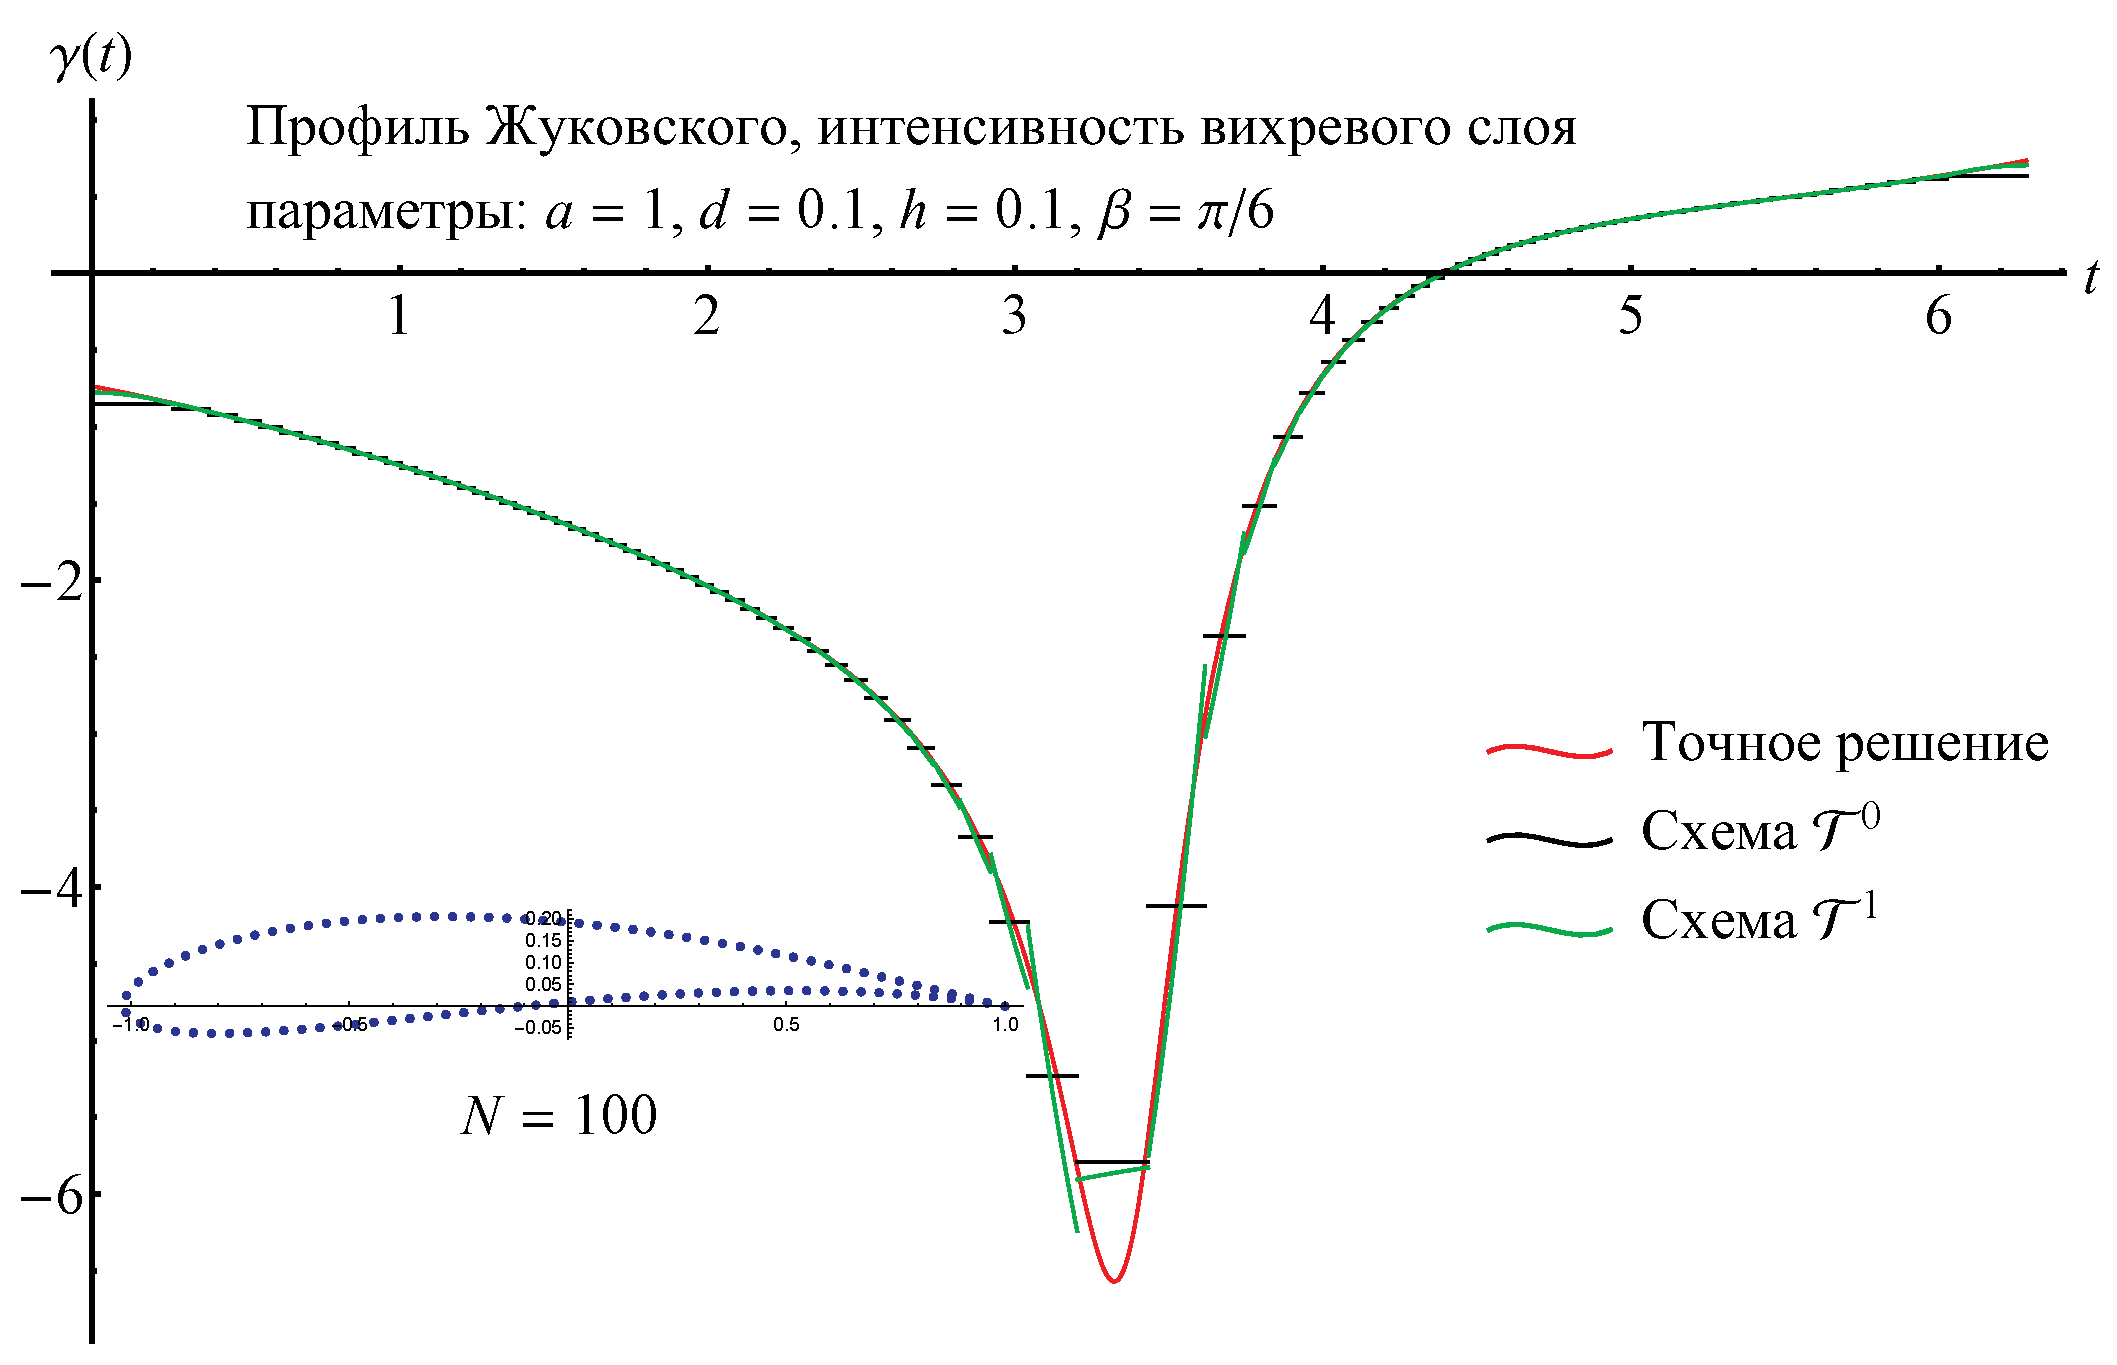
\includegraphics[width=0.9\textwidth]{wing100boundSol_toYuliya}
		%\column{0.5\textwidth}
		%	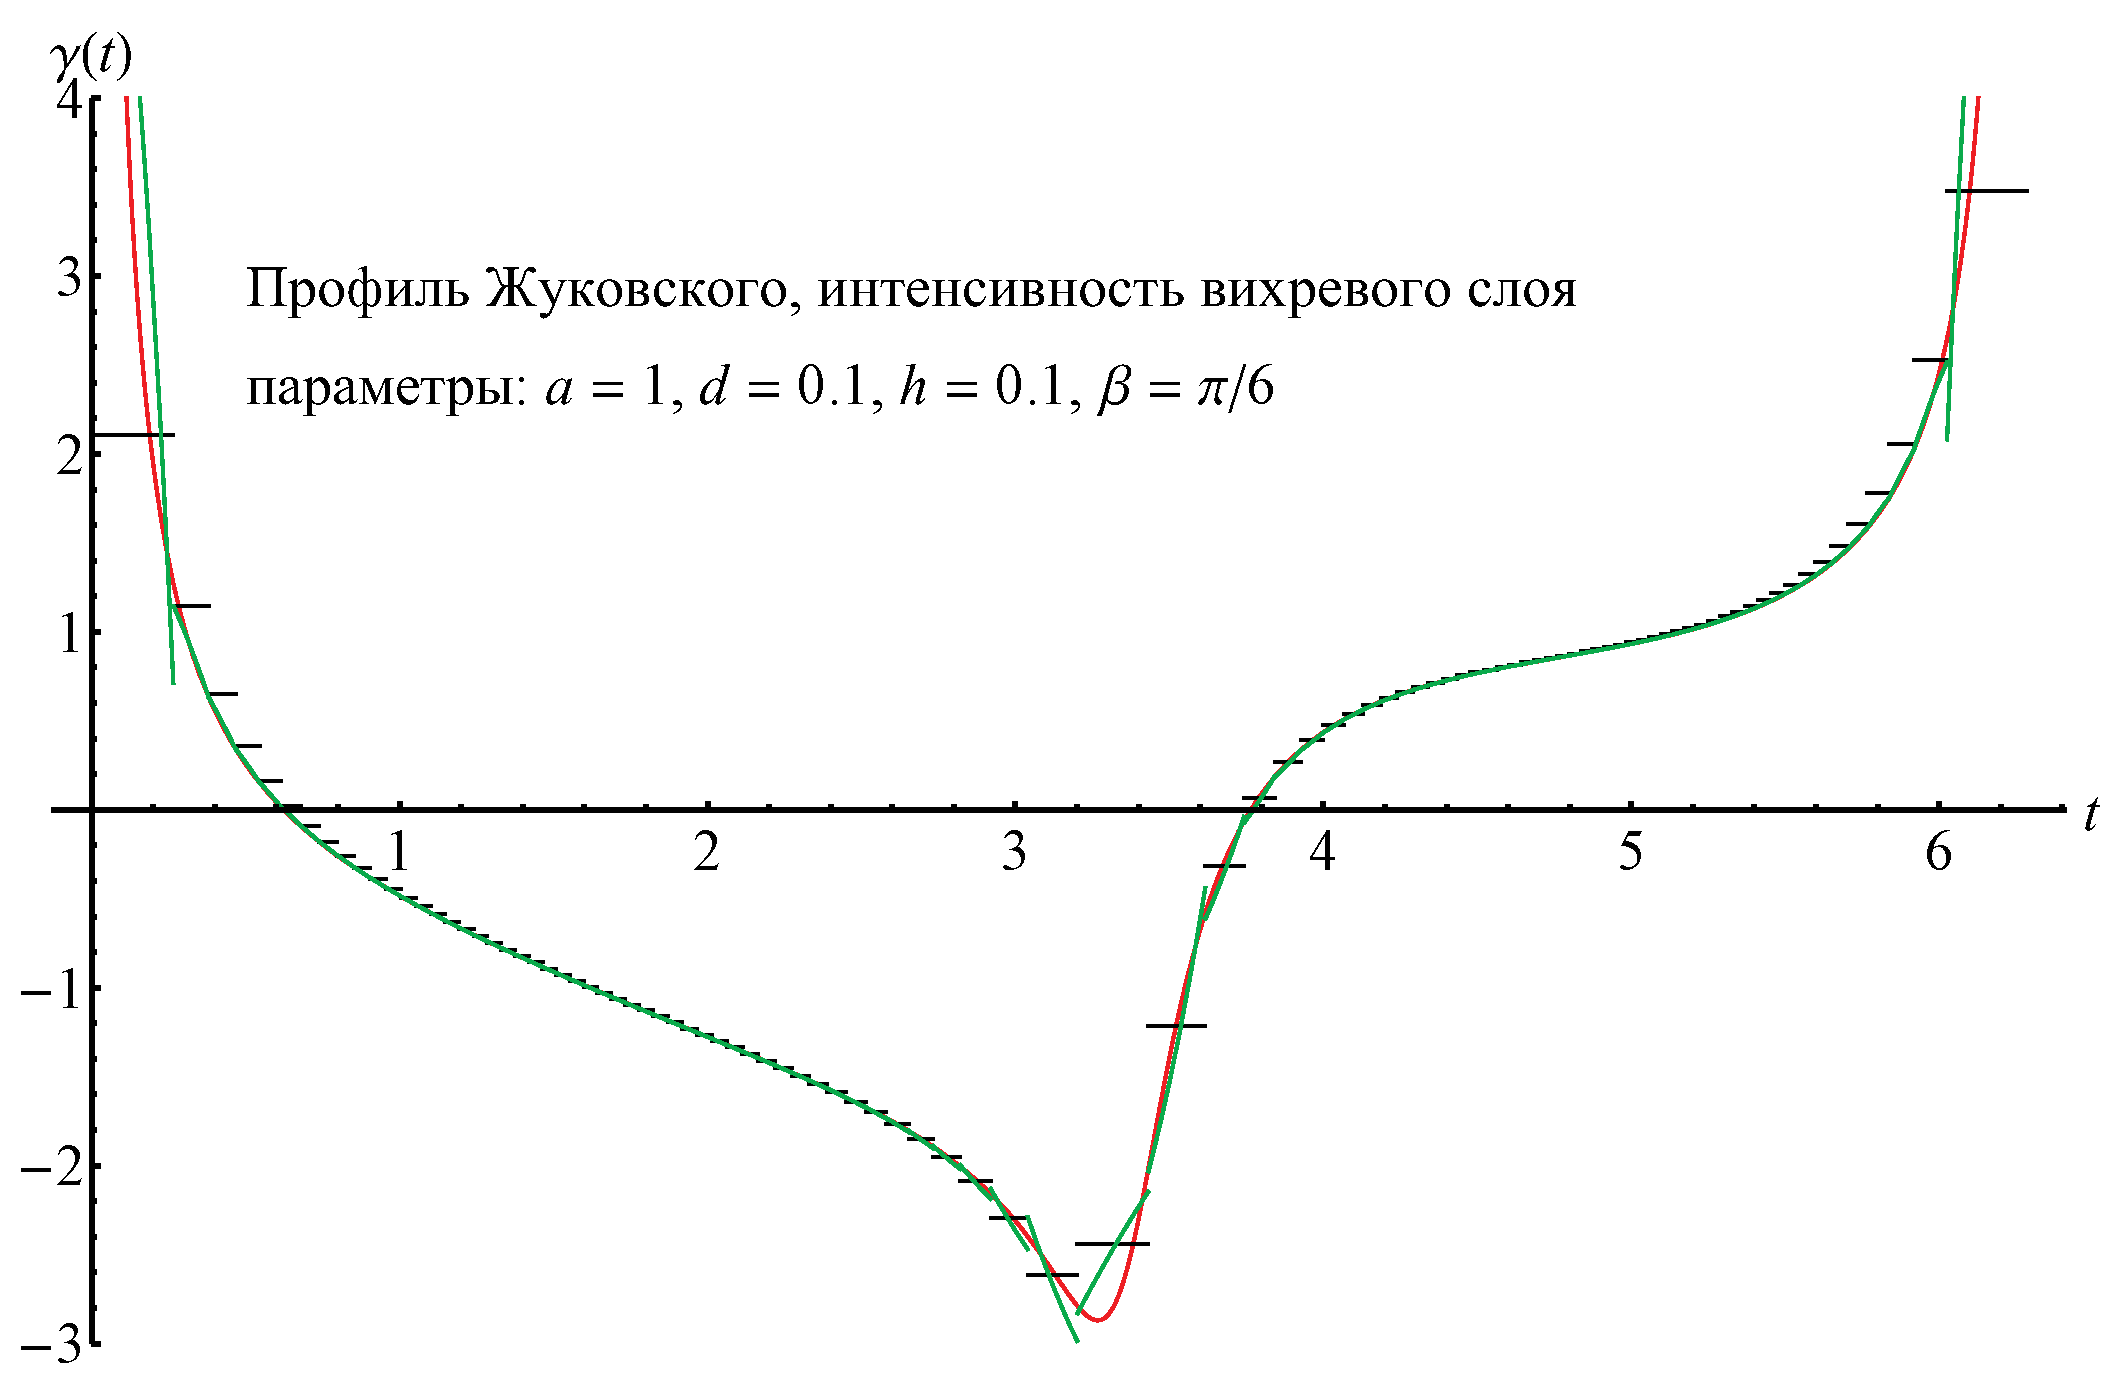
\includegraphics[width=\textwidth]{wing100unboundSol_toYuliya}
\end{frame}
\begin{frame}{Результаты применения схем}
	Суммарная циркуляция $\Gamma^{\ast}=0$, что соотвествует нестационарному обтеканию крыла.	
	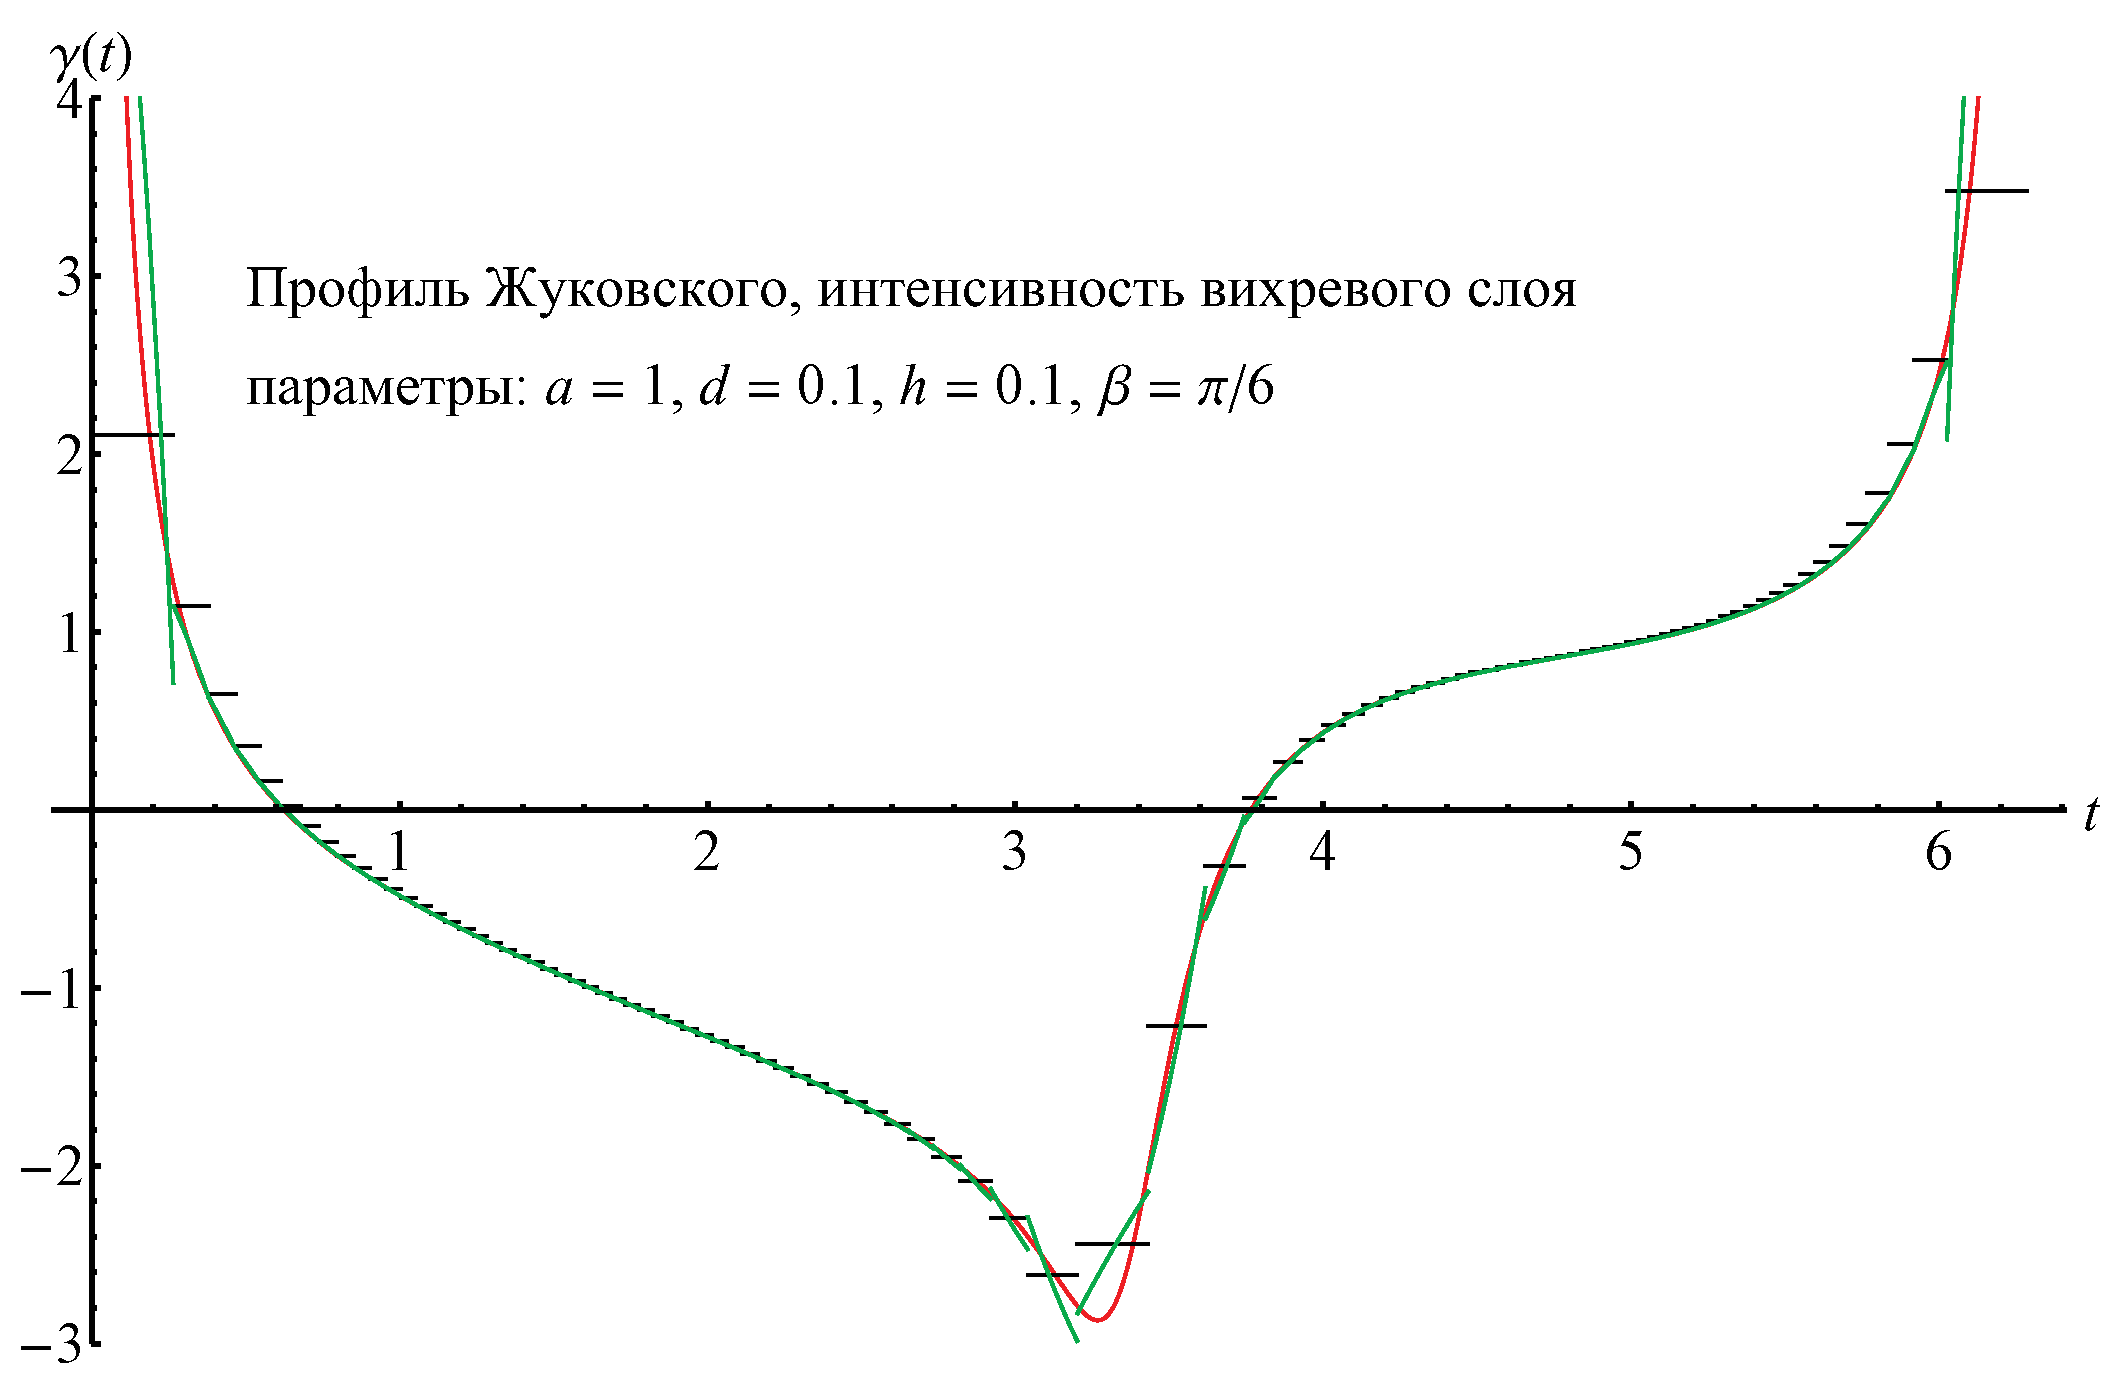
\includegraphics[width=0.9\textwidth]{wing100unboundSol_toYuliya}
\end{frame}

\section{$T$-схема с асимптотическим решением}
\begin{frame}{$T$-схема с асимптотическим решением}
	\begin{columns}\vspace*{-3.5mm}
		\column{0.67\textwidth}
			Для неограниченных решений на крайних панелях вводим базисные функции:
		\begin{gather*}
		\vspace*{-4.5mm}
			\varphi_1^{a}(\vec r)=\frac{L_1^\mu}{s_1(\vec r)^{\mu}}-\frac{1}{1-\mu},\quad \mu=1-\frac{\pi}{\chi},\\
			\bar{\varphi}_n^{a}(\vec r)=\frac{L_n^\mu}{\bigl(L_n-s_n(\vec r)\bigr)^{\mu}}-\frac{1}{1-\mu}.
		\end{gather*}\vspace*{-0.5mm}
		Асимптотика: $\gamma(\rho)=\rho^{-\mu}$.\\
		Коэффициенты схемы найдены аналитически при $\chi=p/q$, $p$, $q\in \mathbb{N}$.
		\begin{columns}
		\column{0.5\textwidth}
		\includegraphics[width=\textwidth]{ris10}
		\column{0.5\textwidth}
		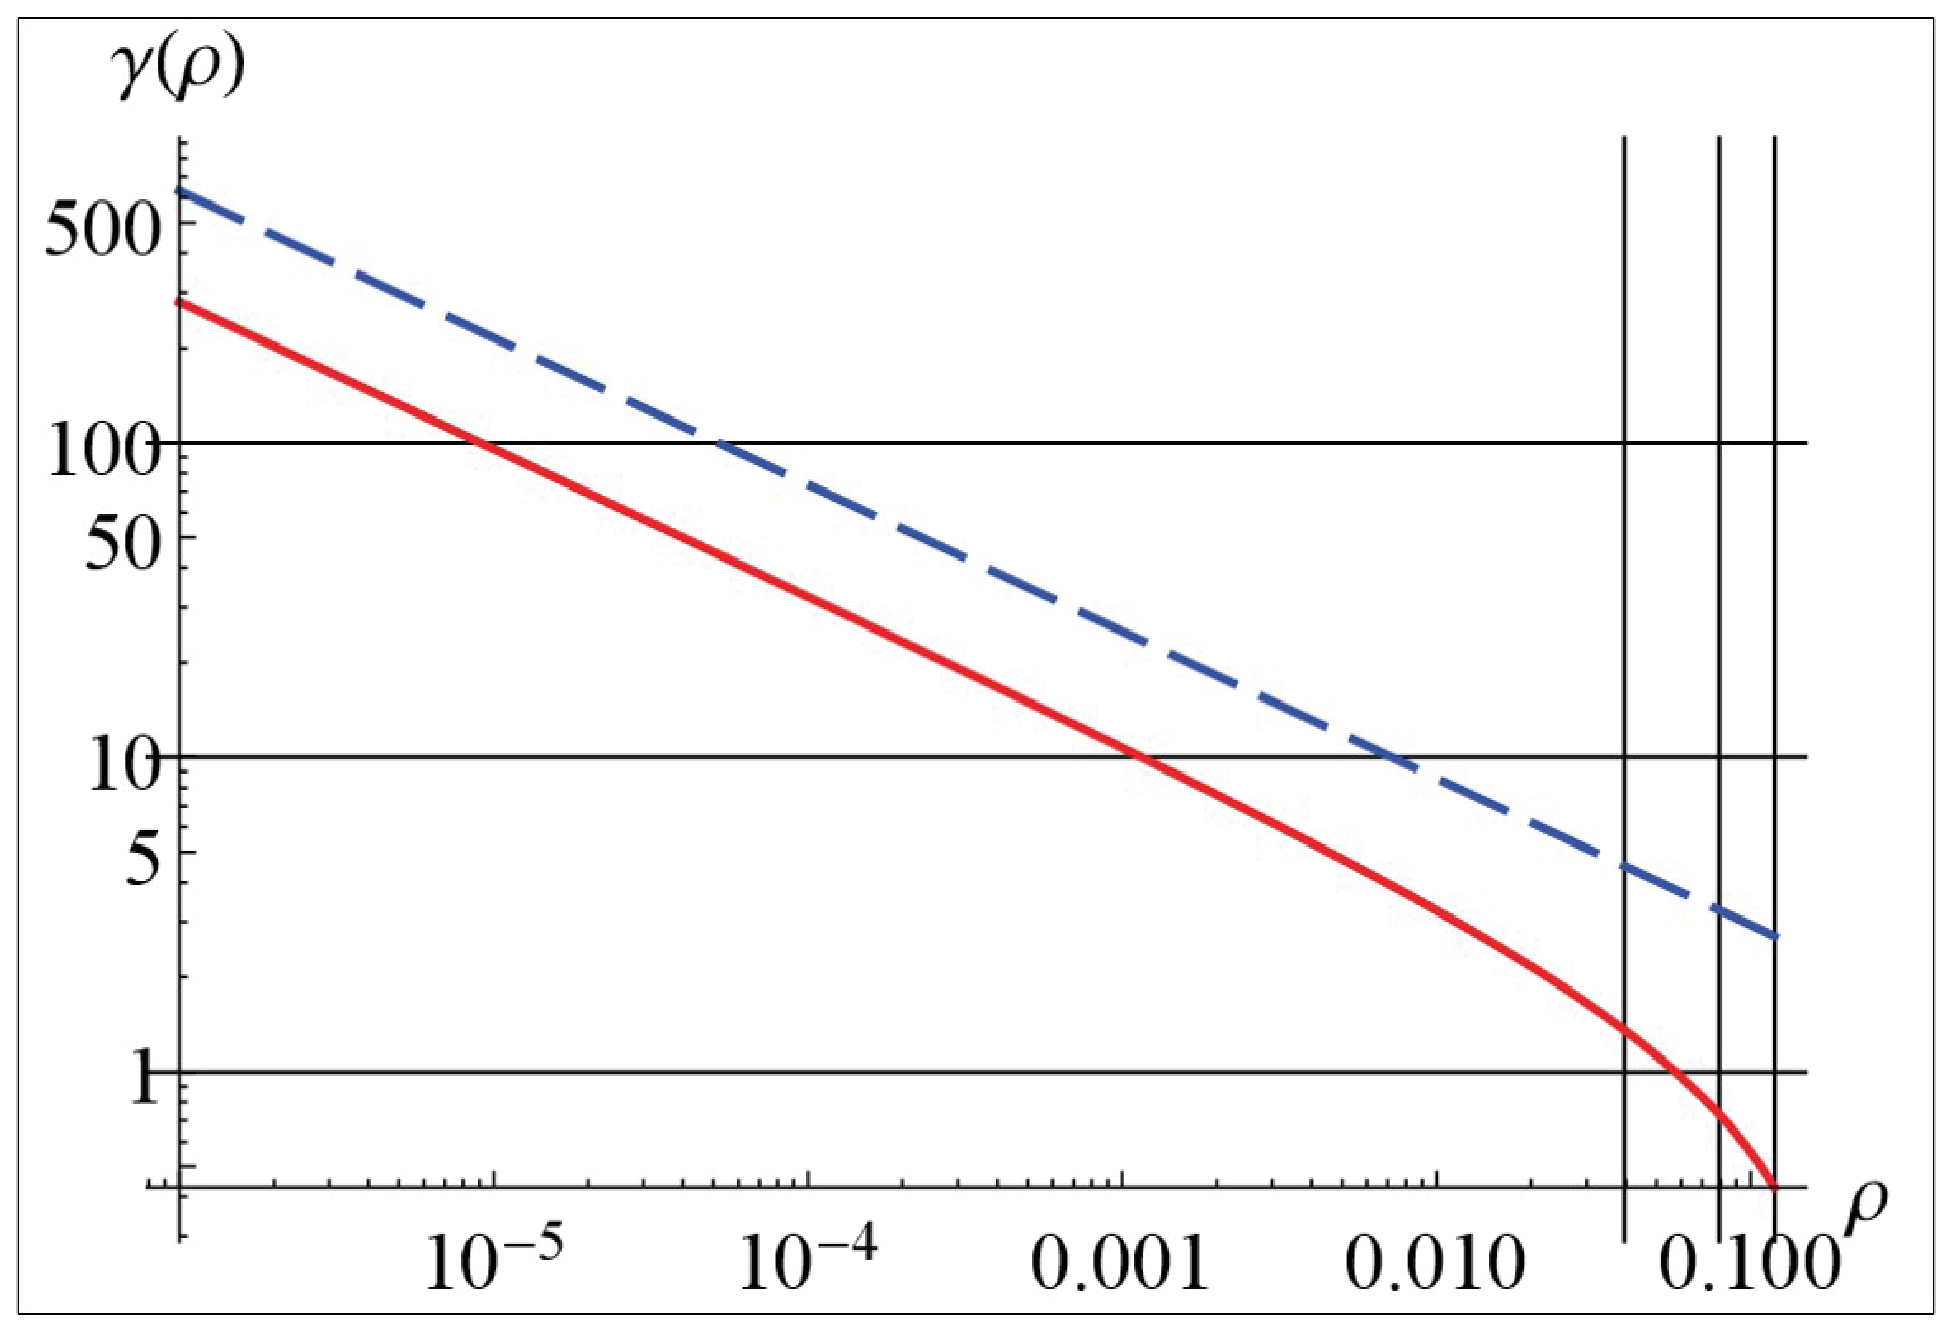
\includegraphics[width=\textwidth]{ris11}
		\end{columns}
		\column{0.4\textwidth}
		\includegraphics[width=0.8\textwidth]{ris8}
		\includegraphics[height=\textwidth]{ris9}
	\end{columns}
\end{frame}


%\begin{frame}
%	Правая часть системы имеет вид
%	\[
%	b_i^p = \frac{1}{L_i} \int_{K_i} \bigl( \vec f(\vec r) \cdot \vec\tau(\vec r) \bigr) \phi_i^p(\vec r)\, dl_r = (b_V)_i^p + \underbrace{(b_\Omega)_i^p}_0 + (b_{att})_i^p,
%	\]
%	где\vspace*{-2.6mm}
%	\begin{gather*}
%	(b_V)_i^p = \frac{1}{L_i} \vec\tau_i \cdot \int_{K_i} \bigl( \alpha(\vec r) \vec U_K(\vec r) - \vec V_\infty \bigr) \phi_i^p(\vec r)\, dl_r,\\[4mm]
%	(b_{att})_i^p = -\frac{1}{L_i} \vec\tau_i \cdot \int_{K_i} \biggl( \oint_{K} \frac{\vec k \times (\vec r - \vec \xi)}{2\pi|\vec r - \vec \xi|^2}\gamma^{att}(\vec\xi)\,dl_\xi
%	+\oint_{K} \frac{q^{att}(\vec \xi) (\vec r - \vec \xi)}{2\pi|\vec r - \vec \xi|^2}\,dl_\xi  \biggr)\phi_i^p(\vec r)\, dl_r.
%	\end{gather*}
%	\begin{block}{}
%		\[
%		\begin{array}{@{}l@{\qquad}l@{}}
%		(\gamma^{att})_i^0 = \vec U_K(\vec c_i) \cdot \vec \tau_i,  &
%		(\gamma^{att})_i^1 = \dot L_i=0,\\
%		(q^{att})_i^0 = \vec U_K(\vec c_i) \cdot \vec n_i,  &
%		(q^{att})_i^1 = -L_i \omega_i.
%		\end{array}
%		\]		
%	\end{block}	
%\end{frame}	

%\begin{frame}
%	Примеры нахождения решения с использованием кусочно-линейной схемы для единичной окружности и для профиля Жуковского с параметрами  $a=1.0$, $d=0.1$, $h=0.1$, углом атаки $\beta=\pi/6$.
%	\begin{columns}
%		\begin{column}{0.5\textwidth}
%			\begin{figure}[!h]\vspace*{-4mm}
%				\includegraphics[width=\textwidth]{circlelin}
				%\caption{$n=40$}
%			\end{figure}
%			\includegraphics[width=0.6\textwidth]{strlinesCircle}
%		\end{column}	
%		\begin{column}{0.6\textwidth}
%			\begin{figure}[!h]\vspace*{-4mm}
%				\includegraphics[width=\textwidth]{zhklin}
%				%	\caption{$n=100$}
%			\end{figure}
%			\includegraphics[width=0.6\textwidth]{strlineAirfoilWithoutVort0}
%		\end{column}
%	\end{columns}	
%\end{frame}

\begin{frame}{$T$-схема с асимптотическим решением}
	\begin{block}{}
		\begin{itemize}
			\item Новые базисные функции вводятся только на крайних панелях.
			\item Проекционные функции совпадают с базисными функциями кусочно-линейной $T$-схемы.
		\end{itemize}
	\end{block}
Окончательная СЛАУ
	\begin{equation*}
	\begin{pmatrix}
		[A^{00}] + [D^{00}] & [A^{01}] + [D^{01}] & \{I_n\} \\
		[A^{10}] + [D^{10}] & [A^{11}] + [D^{11}] & \{O_n\}\\
		\{L^0\}^{\mathrm{T}} & \{L^1\}^{\mathrm{T}} & 0
	\end{pmatrix}
	\label{sys2}
%	\left(
%	\begin{array}{@{}ccc@{}}
%	A^{00} + D^{00} & A^{01} + D^{01} & I_n \\
%	[A^{10}] + [D^{10}] & [A^{11}] + [D^{11}] & \{O_n\}\\
%	\{L^0\}^{\mathrm{T}} & \{L^1\}^{\mathrm{T}} & 0
%	\end{array}
%	\right)
	\left(
	\begin{array}{@{}c@{}}
	\{\gamma^0\}\\
	\{\gamma^1\}\\
	R
	\end{array}
	\right)
	=
	\left(
	\begin{array}{@{}c@{}}
	\{b^0\} \\
	\{b^1\}\\
	\Gamma^\ast
	\end{array}
	\right),
	\end{equation*}
совпадает по форме с системой для кусочно-линейной $T$-схемы. Все коэффициенты системы остаются неизменными за исключением первых и последних столбцов блоков $[A^{01}]$ и $[A^{11}]$, а также первого и последнего диагональных коэффициентов в блоке $[D^{11}]$.	
\end{frame}

\section{Присоединенные массы}
\begin{frame}{Присоединенные массы}
\begin{block}{}
	 Задача вычисления присоединенных масс $\lambda_{ij}$, $i,\,j=1,\,\ldots,\,6$, $\Leftrightarrow$ задаче о восстановлении шести потенциалов течения $\Phi_i(\vec r)$ и последующему вычислению интегралов
	\[
	\lambda_{ij} = -\rho \oint_S \Phi_i(\vec r) \frac{\partial \Phi_j(\vec r)}{\partial \vec n} dS,
	\]
	где $\Phi_i(\vec r)$ --- потенциал, соответствующий движению тела с единичной скоростью в направлении $i$-й координатной оси для $i=1,\,2,\,3$ или вращению с единичной угловой скоростью вектор которой направлен вдоль $(i-3)$-й координатной оси для $i=4,\,5,\,6$; $\vec n$ --- единичный орт внешней к поверхности тела нормали.
\end{block}	
\end{frame}	

\begin{frame}
	\begin{columns}
		\begin{column}{0.65\textwidth}
			\[
			[\Lambda]=
			\begin{pmatrix}
			\lambda_{11} & \lambda_{12} & \lambda_{16} \\
			& \lambda_{22} & \lambda_{26} \\
			&              & \lambda_{66} \\
			\end{pmatrix}
			\]
			\begin{block}{}
			\begin{gather*}
			\label{addmass}
			{\lambda}_{j} = \rho \oint_S \vec r \times \bigl( \vec\gamma_j(\vec r) + \vec\gamma_j^{att}(\vec r) \bigr)dS,\\[0.4mm]
			\label{addmoment}
			{\mu}_{j 6} = -\frac{\rho}{2} \oint_S |\vec r - \vec r_0|^2 \bigl( \vec\gamma_j(\vec r) + \vec\gamma_j^{att}(\vec r) \bigr)dS,
			\end{gather*}
			где $\lambda_{j} = \bigl(\lambda_{1j},\,\,\lambda_{2j}\bigr)^T$;
				
			$\vec r_0$ --- радиус-вектор точки, относительно которой вычисляются моменты.
			\end{block}
		\end{column}
	\begin{column}{0.4\textwidth}
	Отобразим внешность круга радиусом $\eta a$, с центром в точке $z_c = a\bigl(\eta e^{i \alpha} - 1\bigr)$ на внешность профиля $\zeta$ согласно закону
		\[
		\zeta(z) = e^{-i \alpha} \Bigl(z + \frac12 \Bigl( z + \frac{a^2}{z}\Bigr)\Bigr),
		\]
		\begin{figure}[!h]
			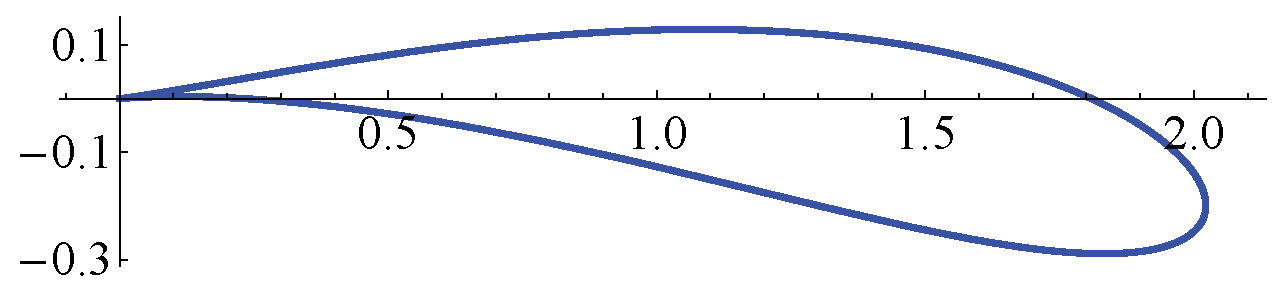
\includegraphics[width=\textwidth]{figWing}
		\end{figure}
	\end{column}
	\end{columns}
\end{frame}

\begin{frame}
	Точные значения присоединенных масс с учетом $\sigma = \eta/(2\eta\cos\alpha - 1)$, $\rho$ "--- плотность среды:
	\begin{gather*}
	\lambda^{\mathrm{ex}}_{11} = \frac{\pi \rho a^2}{4}\bigl(\sigma^2 + \eta^2 - 2\cos2\alpha\bigr), \qquad
	\lambda^{\mathrm{ex}}_{22} = \frac{\pi \rho a^2}{4}\bigl(\sigma^2 + \eta^2 + 2\cos2\alpha\bigr), \qquad
	\lambda^{\mathrm{ex}}_{12} = \frac{\pi \rho a^2}{2}\sin 2\alpha, \\
	\lambda^{\mathrm{ex}}_{16} = \frac{\pi \rho a^3}{8} \sin\alpha \bigl( \sigma^2 + \eta^2 + 4(\sigma+\eta)\cos\alpha \bigr), \\
	\lambda^{\mathrm{ex}}_{26} = \frac{\pi \rho a^3}{8} \bigl( \sigma^3 + \eta^3 + ( \sigma^2 + \eta^2)\cos\alpha  + 2(\sigma+\eta)\cos2\alpha \bigr),\\
	\lambda^{\mathrm{ex}}_{66} = \frac{\pi \rho a^4}{8} \sigma^2 \eta^2 \bigl( 8\sigma^2 \eta^2 \cos^4\alpha - 2 \sigma \eta \sin^2 2\alpha + \cos4\alpha \bigr).
	\end{gather*}
\end{frame}


%	\begin{table}[!h]
%		\label{accuracy}
		%\caption{Число панелей, гарантирующих достижение заданной точности}\medskip
%		\centering
%		%% \tablesize{} %% You can specify the fontsize here, e.g., \tablesize{\footnotesize}. If commented out \small will be used.
%		\begin{tabular}{|c|c|c|}
%			\hline
%			&  \textbf{Кусочно-постоянная}	& \textbf{Кусочно-линейная}\\
%			& \textbf{схема} & \textbf{схема} \\
%			\hline
%			1\,\%    & 265    & 66\\
%			0{.}1\,\% & 3\,700 & 307\\
%			\hline
%		\end{tabular}
%	\end{table}
	
%\begin{frame}{}
%	Ошибки при вычислении присоединенных масс:
%	\begin{table}[!h]
	%\centering			
%		\begin{tabular}{|c|c|c|c|с|}
%			\hline
%			$n$ & 400 & 800 & 1600 & 3200 \\\hline
%			%Кус.-лин. схема & $0.000739$ & $0.000351$ & $0.000171$ & $0.000085$\\
%			\hline
%			%Асимпт. схема &  $0.000301$ & $0.000076$ & $0.000019$ & $4.74\times10^{-6}$ \\
%			\hline
%		\end{tabular}
%	\end{table}	
%	Порядки сходимости схем:
%	\begin{table}[!h]
	%\centering			
	%\vspace*{-6mm}			
		%\begin{tabular}{|c|c|c|c|c|с|}
		%	\hline
%			$n$ & 400 & 800 & 1600 & 3200 \\ \hline
			%Кус.-лин. схема &  $1.1586$ & $1.07779$ & $1.03342$ & $1.01161$\\
%			\hline
			%Асимпт. схема & $1.98194$ & $1.99322$ & $1.99743$ & $1.9991$ \\
%			\hline
		%\end{tabular}
%	\end{table}
%\end{frame}


\begin{frame}
	Ошибки при вычислении присоединенных масс:
	\begin{table}[!h]
\centering			
		\begin{tabular}{|c|c|c|c|c|}
			\hline
			$n$ & 400 & 800 & 1600 & 3200 \\\hline
			Кус.-лин. схема & $0.000739$ & $0.000351$ & $0.000171$ & $0.000085$\\
			\hline
			Асимпт. схема &  $0.000301$ & $0.000076$ & $0.000019$ & $4.74\times10^{-6}$ \\
			\hline
		\end{tabular}
	\end{table}	
	Порядки сходимости схем:
	\begin{table}[!h]
\centering						
		\begin{tabular}{|c|c|c|c|c|}
			\hline
			$n$ & 400 & 800 & 1600 & 3200 \\ \hline
			Кус.-лин. схема &  $1.16$ & $1.08$ & $1.03$ & $1.01$\\
			\hline
			Асимпт. схема & $1.98$ & $1.99$ & $2.00$ & $2.00$ \\
			\hline
		\end{tabular}
	\end{table}
\end{frame}

\begin{frame}{Результаты}
	В ходе работы получены следующие результаты
	\begin{block}{}
	\begin{enumerate}
		\item реализована расчетная $T$-схема с  кусочно-линейным и асимптотическим представлениями решения для плоского обтекания гладкого профиля;	
		\item результаты работы каждой из расчетных схем были сравнены с точным решением для профиля Жуковского;
		\item изучена задача о вычислении присоединенных масс и моментов инерции профиля Жуковского по полученному решению относительно интенсивности вихревого слоя на границе профиля.
	\end{enumerate}
	\end{block}	
\end{frame}	
\end{document} 